\chapter{Machine vision}

\Gls{machinevision} is the branch of \Gls{ai} focussed on image processing.
The machine vision task performed in this work is called instance \Gls{segmentation}.
In this chapter, I explain what this means. 
The task of segmentation is compared to other machine vision tasks.

This work investigates the used of \Gls{weaklysupervisedl} data for training an Instance segmentation model. 
The concept and benefits of \Gls{weaklysupervisedl} machine learning are explained.

\section{Machine vision tasks}



\begin{SCfigure}[][htb]
    \centering
    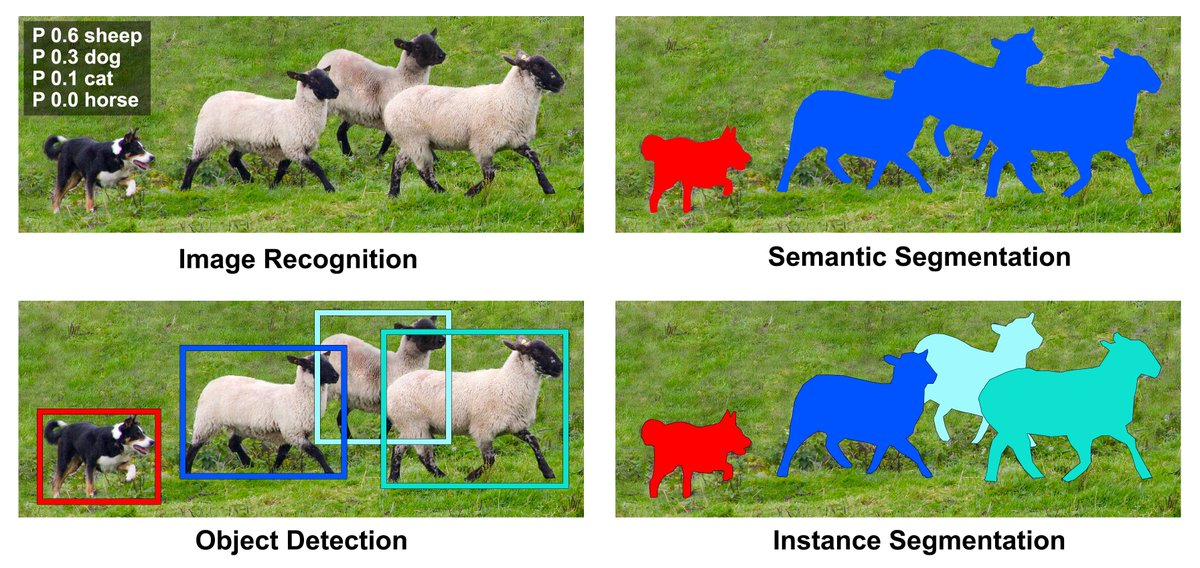
\includegraphics[width=10cm]{/home/thesis/images/Classification_vs_Segmentation.jpg}
    \caption{Illustration to compare different Machine vision tasks \cite{SemTorch76:online}. 
    Object detection means that the location of several objects is estimated by the model. This is indicated by the \textit{bounding boxes}.
    Segmentation of an image is the process of classifying each pixel in the correct class or assign it to the \textit{background} class.
    Semantic segmentation makes no difference between different instances of the same semantic class, instance segmentation does.
    }
\end{SCfigure}

\section{Supervision types}

\begin{SCfigure}[][htb]
    \centering
    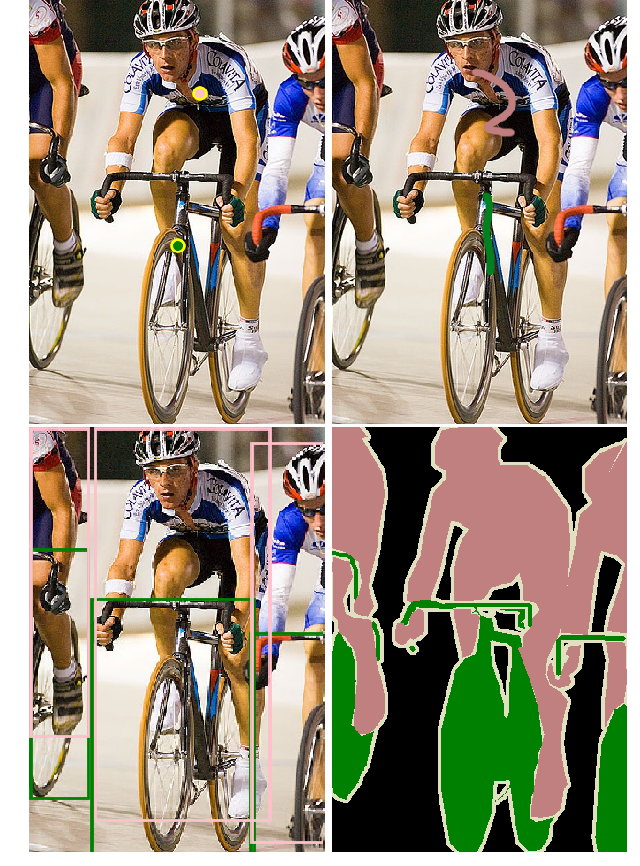
\includegraphics[width=10cm]{/home/thesis/images/McEver.png}
    \caption{Four different annotation types \cite{McEver2020}: 
    On the top left the picture is point level annotated. The points are inflated for visibility.
    On the top right, squiggle annotation is used.
    The bottom left shows bounding box supervion.
    While the bottom right image is fully annotated.
    An image level label would indicate that there are multiple instances of \textit{person} and \textit{bike} in the image.
    }
\end{SCfigure}

\todo[inline]{Motivation of weakly supervised learning --> Difference in annotation time and cost from Bearman and Laradji Covid}